\documentclass[12pt,a4paper]{article}
\usepackage{graphicx, booktabs, siunitx, amsmath, geometry, float}
\usepackage{subcaption}
\usepackage{nicefrac}
\geometry{margin=2.5cm}
\title{Neuromorphic Electronics: VO2 Memristor Characterization}
\author{Gregorio Jaca (U8L9B9)\\\texttt{gregorio.jaca@gmail.com} \and P\'eter Tall\'osy (K14WR1)\\\texttt{peter@tallosy.hu}}
\date{\today}

\begin{document}
\maketitle

\begin{abstract}
This report presents the characterization of volatile vanadium dioxide (VO$_2$) memristors, which exhibit an insulator-metal transition that can be triggered by both temperature and voltage. Measurements were performed on a memristor at row 1, column 3 of the sample array. The I(V) characteristics show the expected hysteretic switching behavior between high-resistance (HRS) and low-resistance (LRS) states. Temperature-dependent resistance measurements reveal the phase transition around \SI{68}{\celsius}, consistent with the known VO$_2$ transition temperature. The results demonstrate the volatile nature of these devices, making them suitable for artificial neuron applications in neuromorphic computing.
\end{abstract}

\section{Introduction}

Neuromorphic electronics aims to implement artificial neural networks in energy-efficient hardware, addressing the growing computational demands of artificial intelligence. Vanadium dioxide (VO$_2$) memristors are volatile devices that can function as artificial neurons due to their hysteretic I(V) characteristics and temperature-dependent insulator-metal transition.

VO$_2$ exhibits a first-order phase transition at approximately \SI{68}{\celsius}, transitioning from an insulating monoclinic phase to a metallic rutile phase. This transition can be triggered thermally or electrically through self-heating in nanoscale devices. The voltage-induced switching shows characteristic set and reset voltages, with the device returning to the high-resistance state at zero bias, making it volatile.

This measurement session focused on characterizing a VO$_2$ memristor device through: (1) circuit validation with series resistor measurements, (2) I(V) curve characterization to identify switching thresholds, (3) temperature-dependent resistance measurements to observe the phase transition, and (4) analysis of the relaxation dynamics.

\section{Results and Discussion}

\subsection{Task 1: Series Resistor Measurement and Circuit Validation}
A series resistor $R_s = \SI{2.17}{\kilo\ohm}$ (measured with multimeter) was connected in series with a surface-mount device (SMD) resistor with nominal value $R_{\text{smd}} = \SI{4.701}{\kilo\ohm}$. The measured value of $R_{\text{smd}} = \SI{4.663}{\kilo\ohm}$ agrees well with the nominal value (within \SI{0.8}{\percent}), validating the measurement circuit and data acquisition system.

\begin{figure}[H]
    \centering
    \begin{subfigure}[t]{0.49\linewidth}
        \centering
        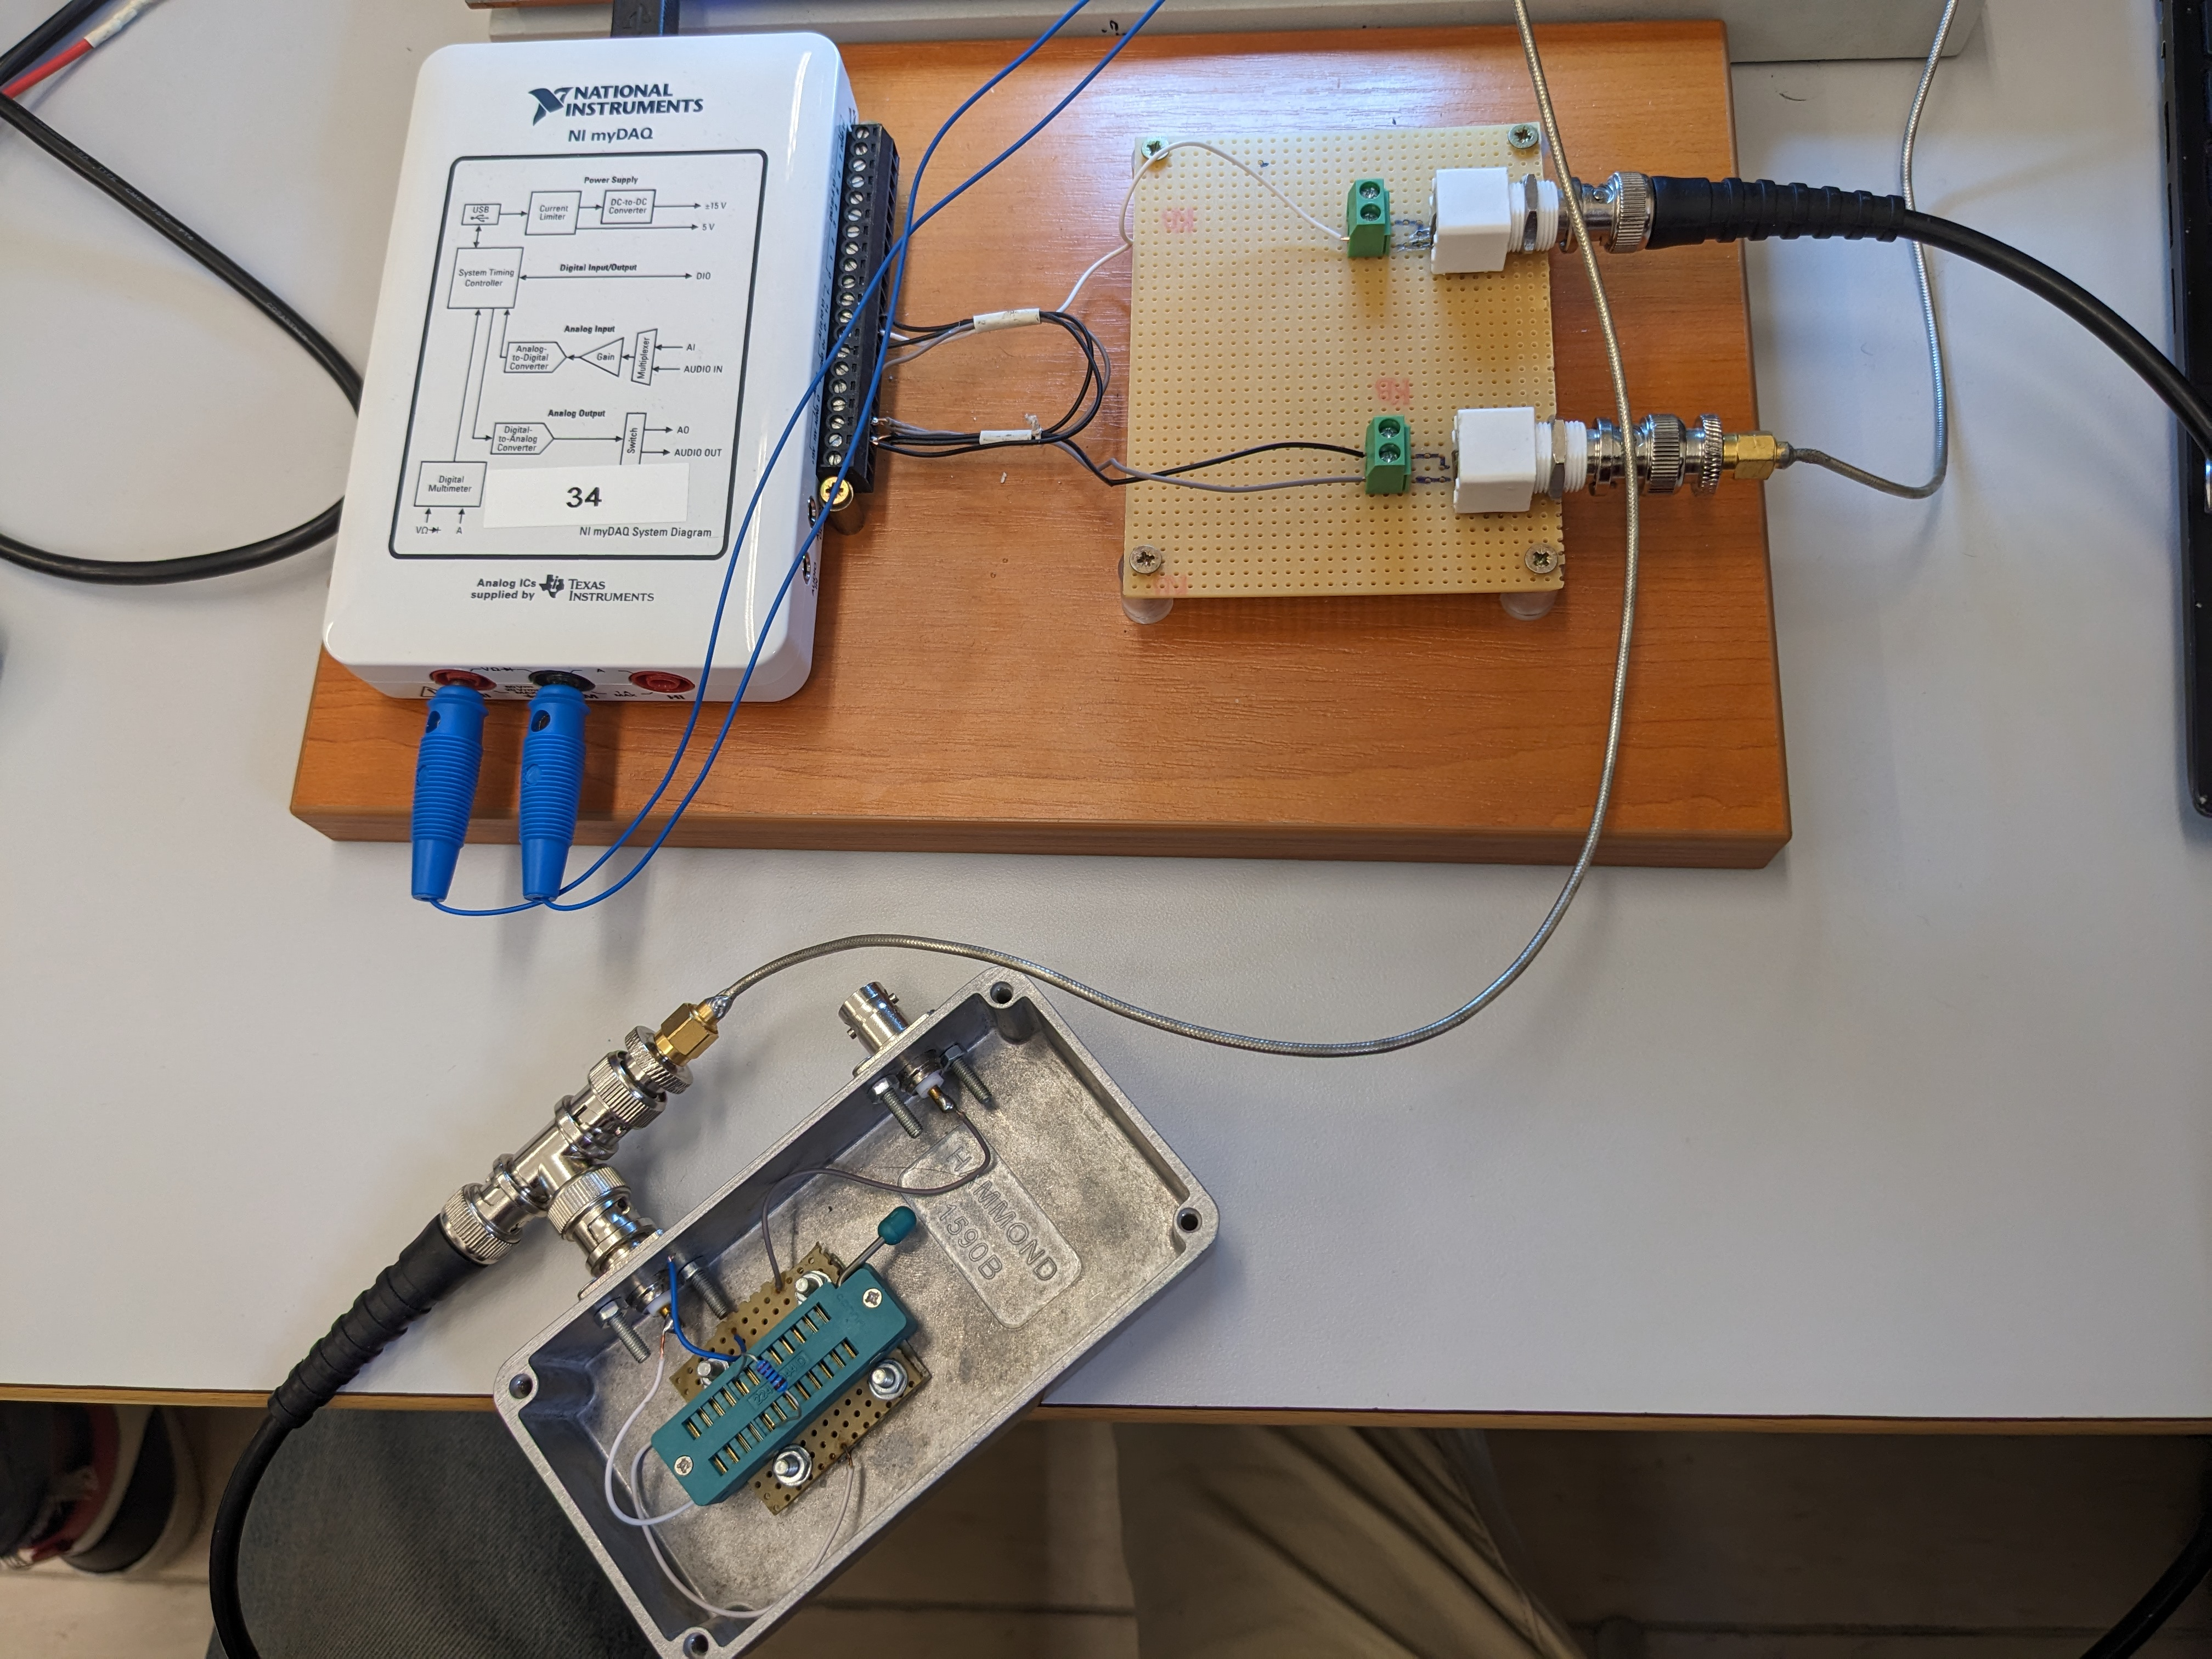
\includegraphics[width=\linewidth]{photos/PXL_20251030_132843909.MP.jpg}
        \caption{Overview of the measurement setup.}
    \end{subfigure}
    \hfill
    \begin{subfigure}[t]{0.49\linewidth}
        \centering
        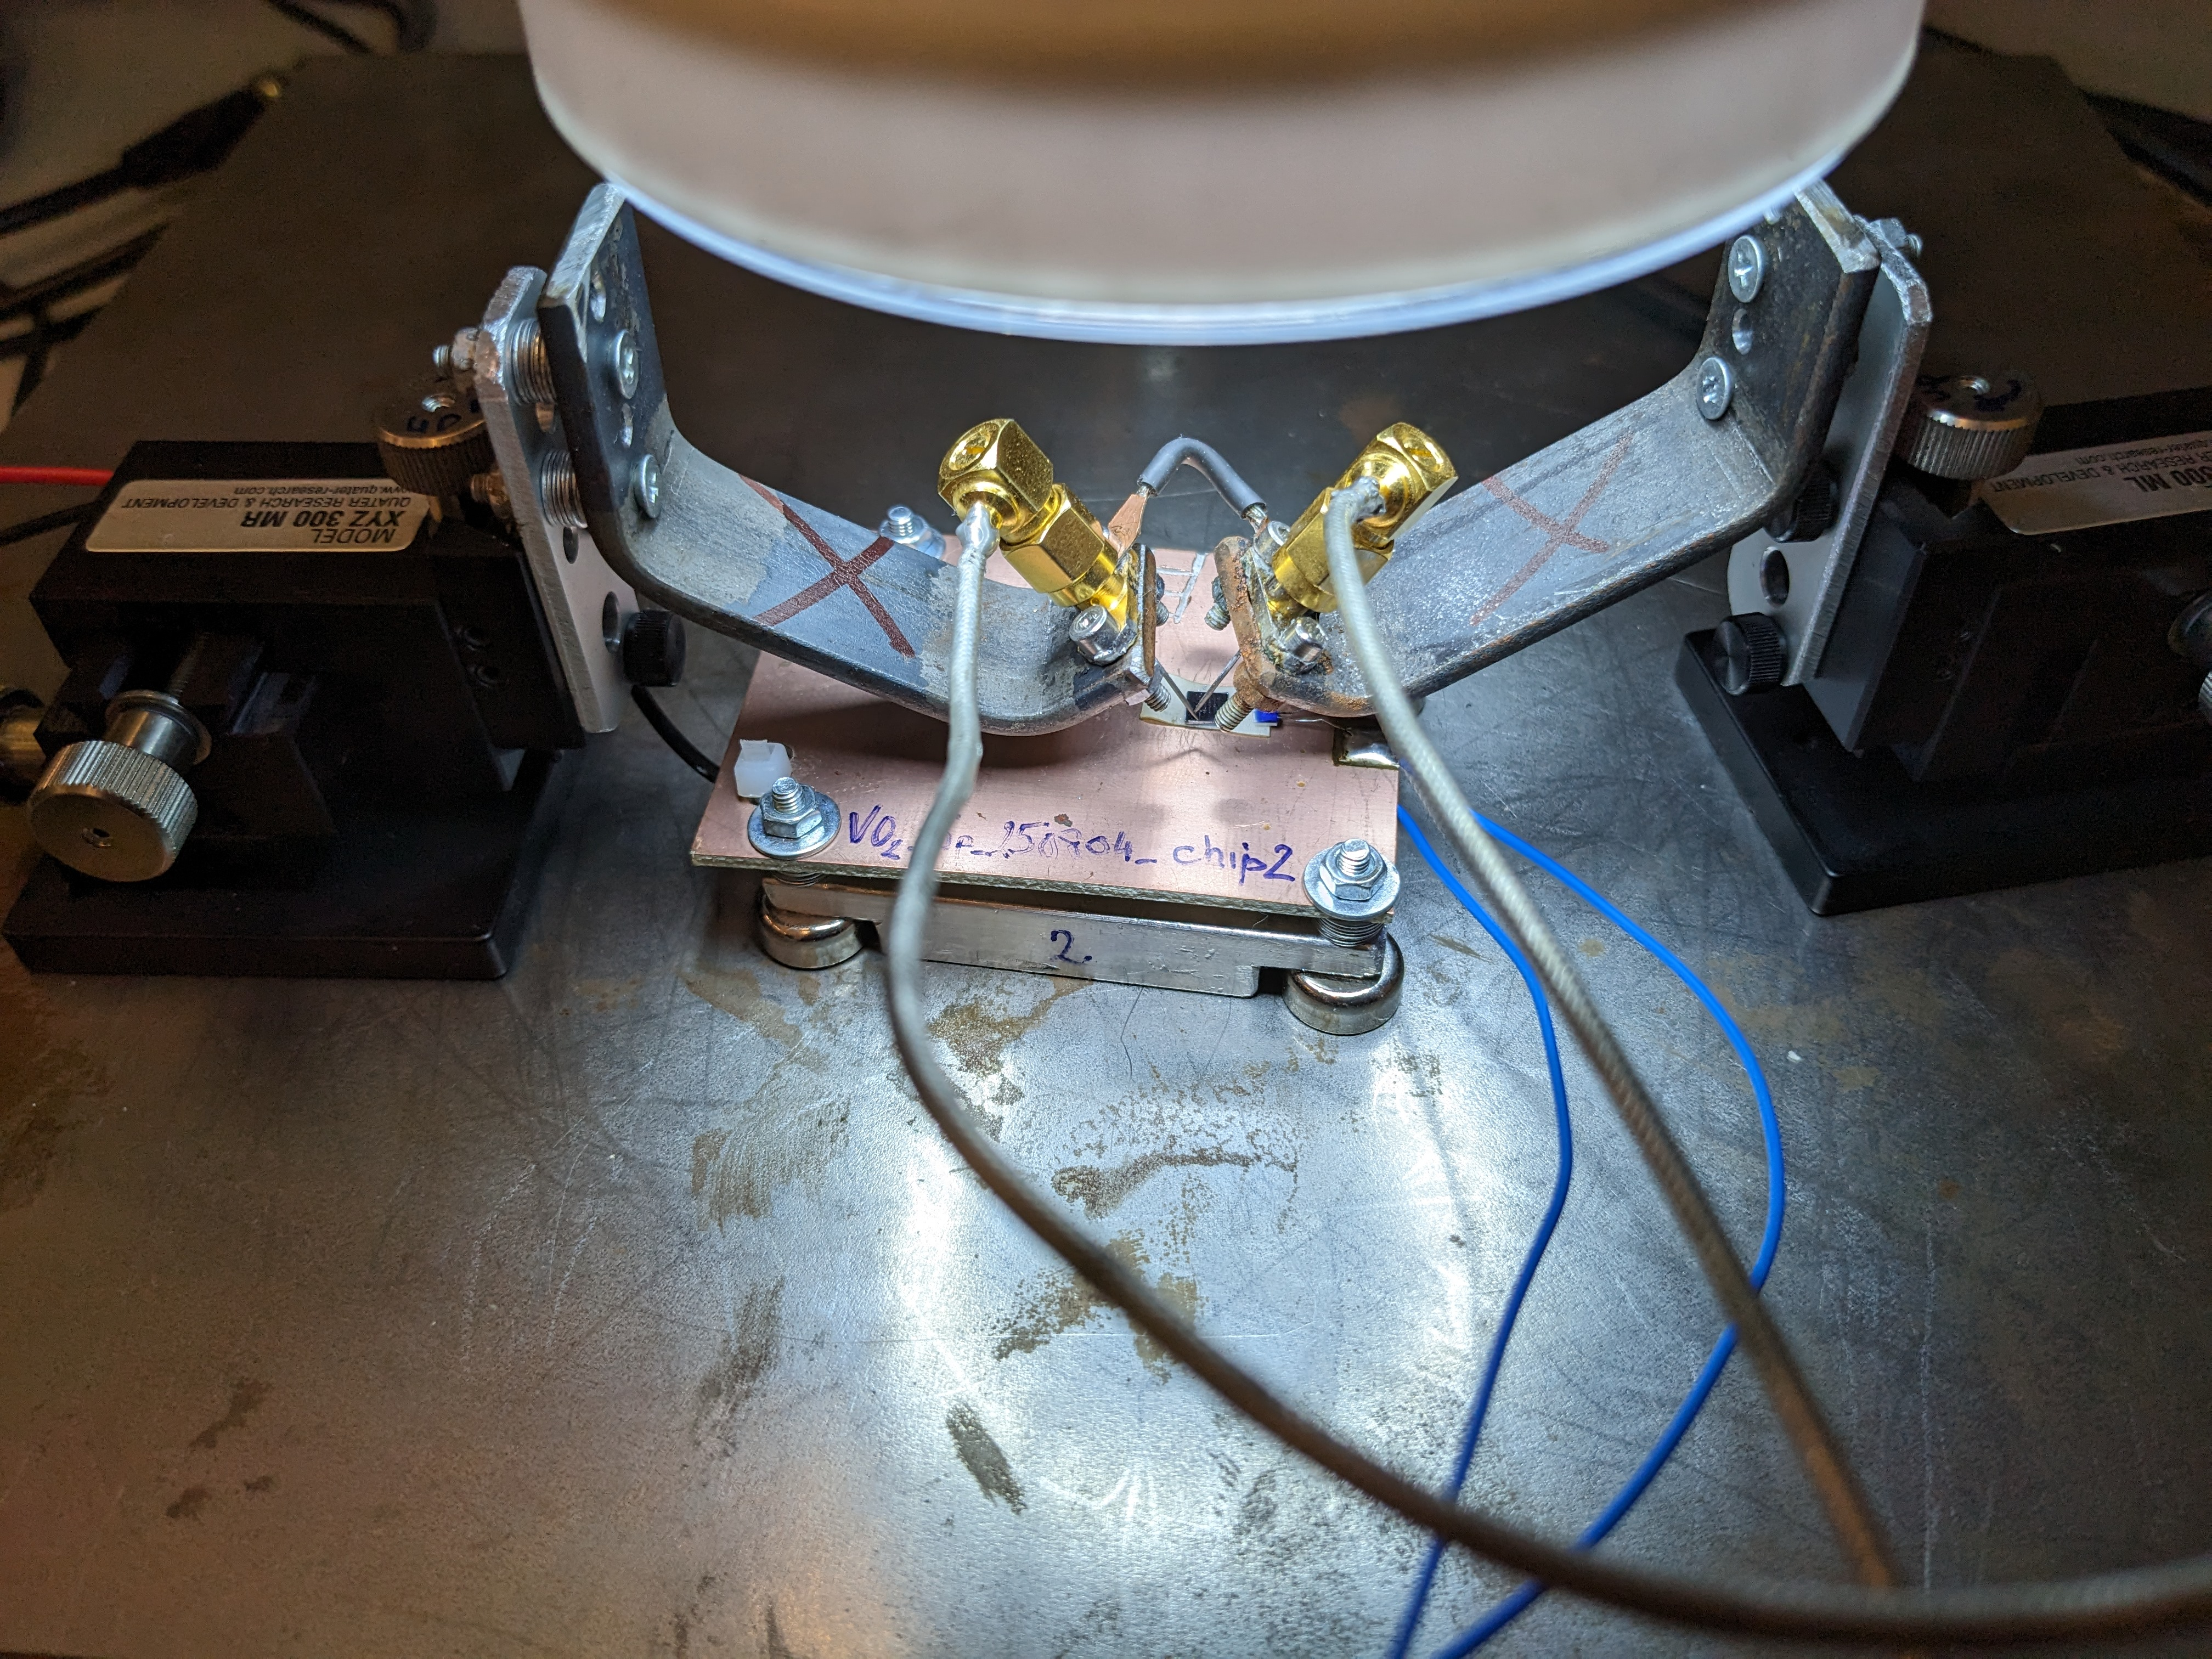
\includegraphics[width=\linewidth]{photos/PXL_20251030_132903116.MP.jpg}
        \caption{Close-up of the VO$_2$ sample chip and probes.}
    \end{subfigure}
    \caption{Measurement setup for circuit validation and device characterization.}
    \label{fig:task1_setup}
\end{figure}

\begin{figure}[H]
    \centering
    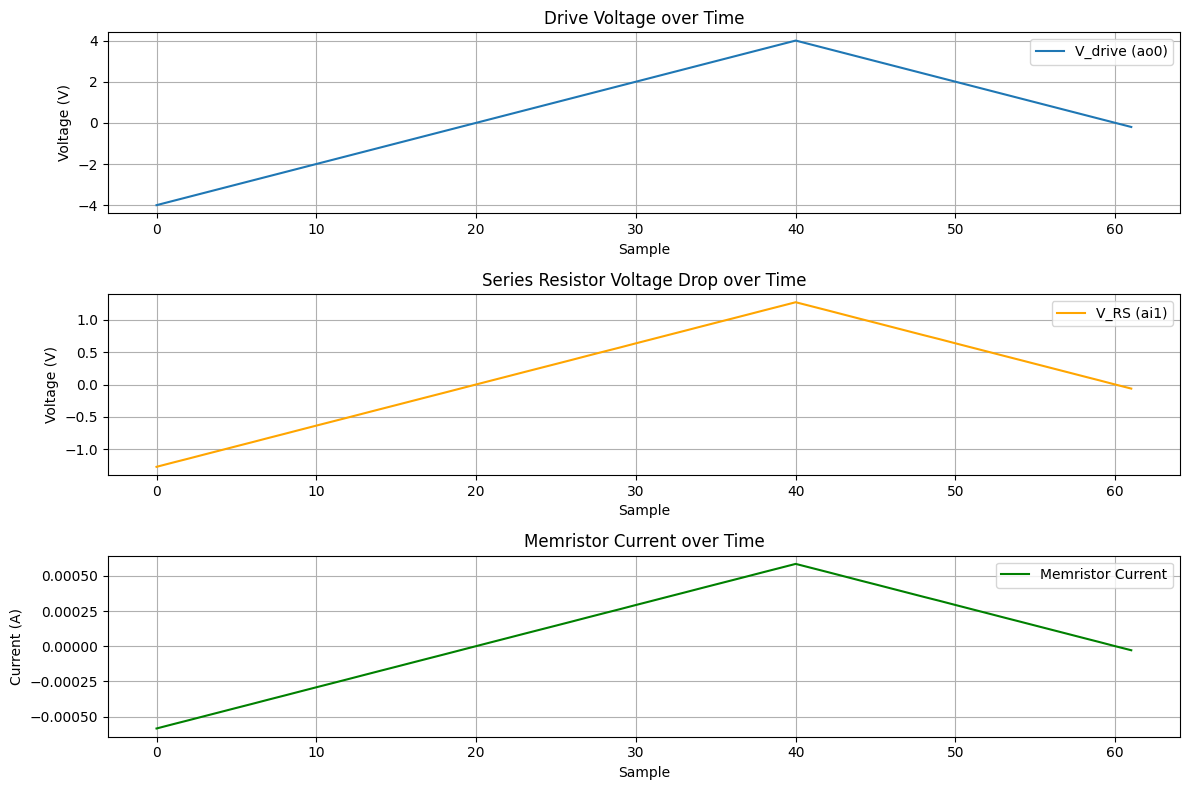
\includegraphics[width=0.6\linewidth]{task1_timeseries.png}
    \caption{Time series of voltage measurements for circuit validation. The stable readings confirm proper circuit assembly and measurement system functionality.}
    \label{fig:task1_timeseries}
\end{figure}

\begin{figure}[H]
    \centering
    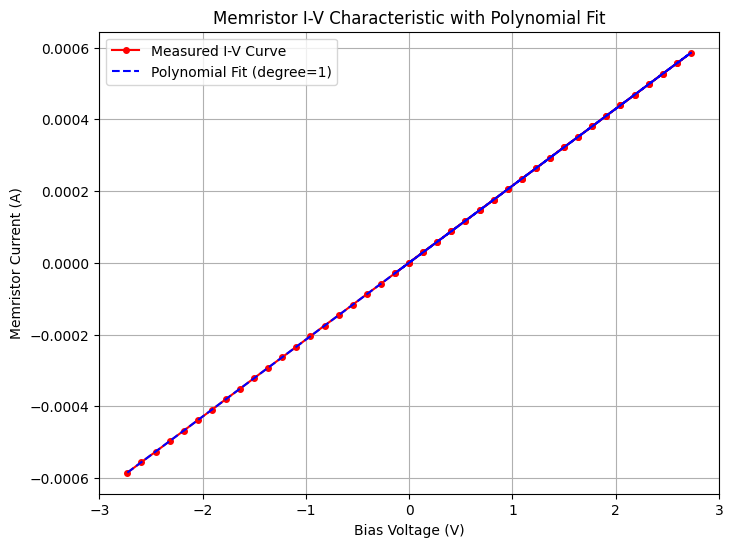
\includegraphics[width=0.6\linewidth]{task1_fit.png}
    \caption{Linear fit to the voltage divider relationship, confirming the expected behavior of the series resistor circuit.}
    \label{fig:task1_fit}
\end{figure}

\subsection{Task 2: I(V) Curve Measurement}

The I(V) characteristics of the VO$_2$ memristor (row 1, column 3) were measured using a voltage ramp from \SI{-4}{\volt} to \SI{+4}{\volt} and back, with a series resistor $R_s = \SI{2.17}{\kilo\ohm}$ to limit current and enable voltage division measurements. The bias voltage across the memristor was calculated as $V_{\text{bias}} = V_{\text{drive}} - I \cdot R_s$, where $I = V_{R_s} / R_s$.

\begin{figure}[H]
    \centering
    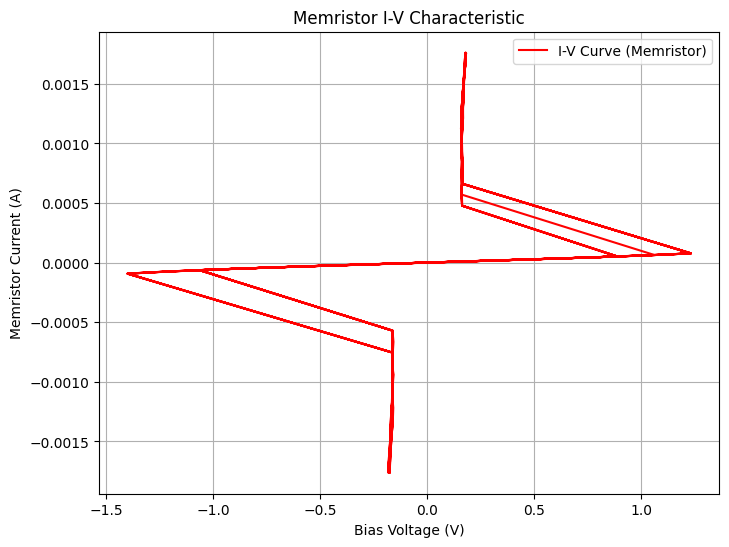
\includegraphics[width=0.6\linewidth]{task2_memristor_iv.png}
    \caption{I(V) characteristic of the VO$_2$ memristor showing hysteretic switching behavior. The device switches from HRS to LRS at the set voltage and returns to HRS at the reset voltage, demonstrating volatile behavior.}
    \label{fig:task2_memristor_iv}
\end{figure}

\begin{figure}[H]
    \centering
    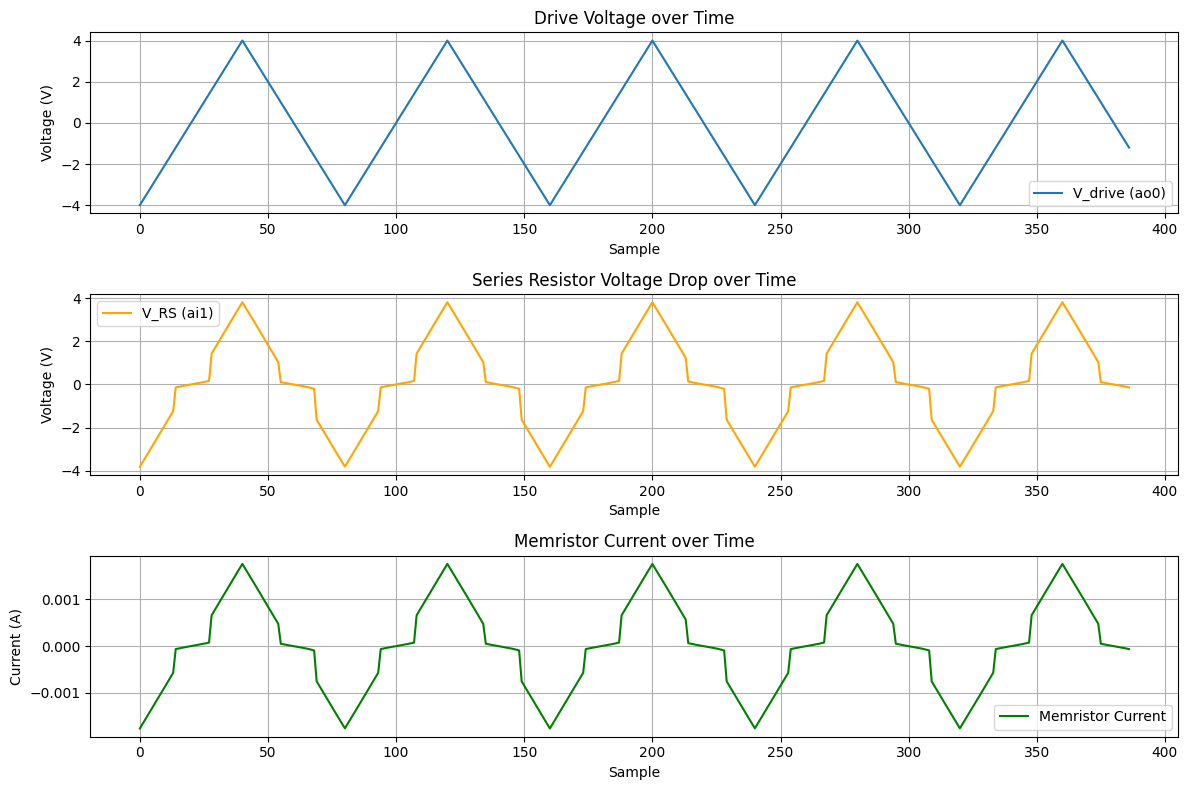
\includegraphics[width=0.6\linewidth]{task_2_three_plots.png}
    \caption{Time-dependent measurements during the I(V) sweep: (top) drive voltage, (middle) series resistor voltage drop, (bottom) calculated memristor current.}
    \label{fig:task2_three_plots}
\end{figure}

The I(V) curve exhibits the expected hysteretic behavior characteristic of VO$_2$ memristors. During the forward sweep (increasing voltage), the device remains in the high-resistance state until reaching the set voltage, where it abruptly switches to the low-resistance state. On the reverse sweep, the device remains in LRS until the reset voltage, where it switches back to HRS. This volatile behavior, where the device always returns to HRS at zero bias, is essential for artificial neuron applications.

The differential resistance $dV_{\text{bias}}/dI$ varies significantly throughout the sweep, reflecting the changing conduction state. In the HRS region, the differential resistance is high (tens of \si{\ohm}), while in the LRS region it decreases substantially. The switching transition itself shows a negative differential resistance region, characteristic of the phase transition.

\subsection{Task 3: Temperature-Dependent Resistance Characteristics}

The resistance of the VO$_2$ memristor was measured as a function of temperature using a Peltier element for heating and cooling, with temperature monitored via a PT1000 resistance thermometer. A constant low bias voltage of \SI{0.2}{\volt} was applied to measure the resistance without triggering voltage-induced switching.

\begin{figure}[H]
    \centering
    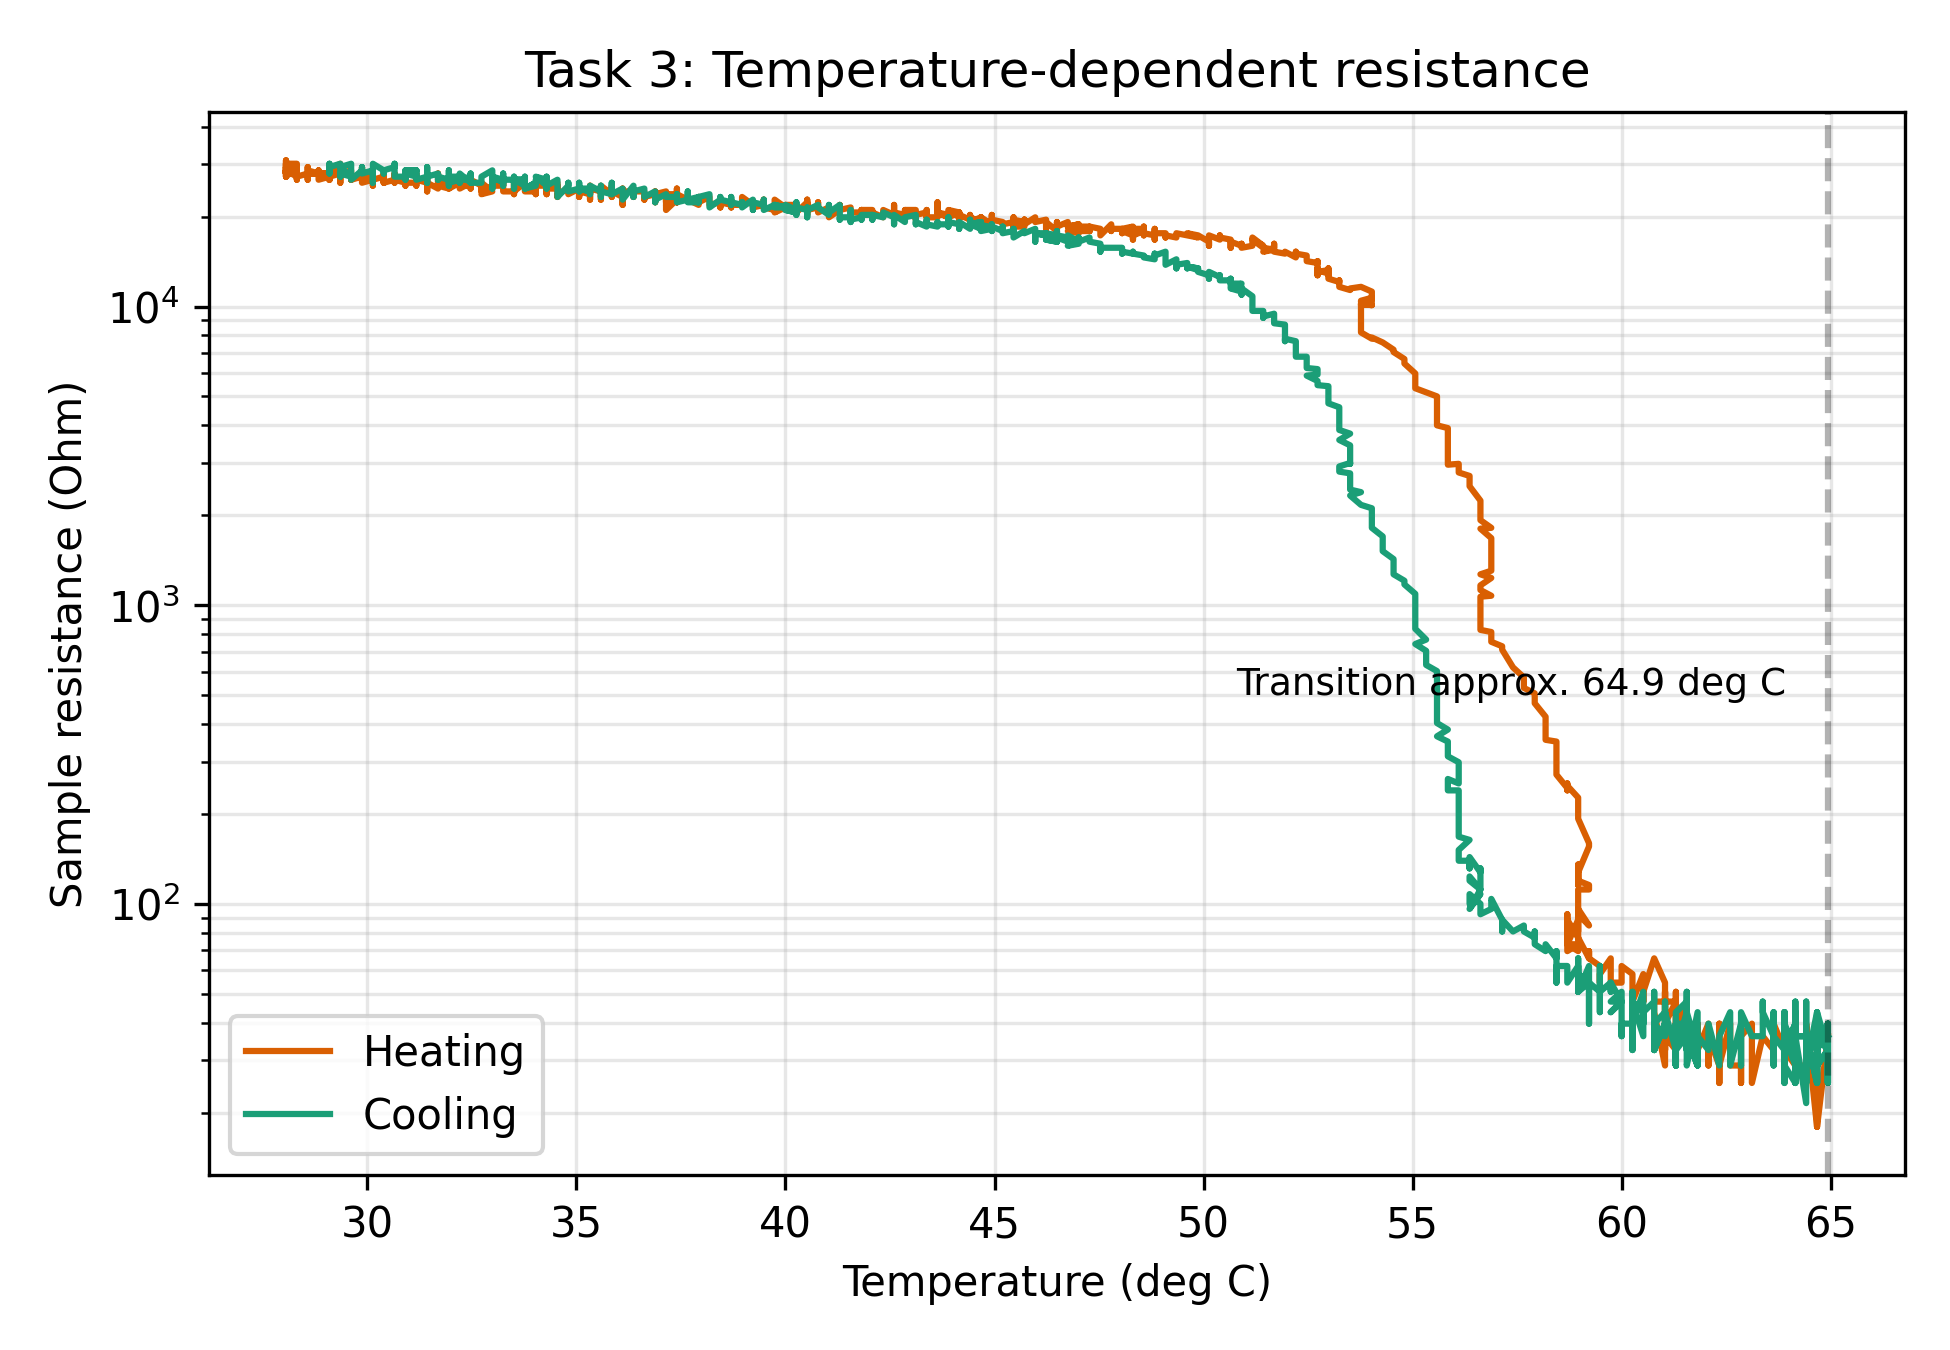
\includegraphics[width=0.7\linewidth]{task3_rt.png}
    \caption{Temperature-dependent resistance extracted from \texttt{task3.csv}. Heating and cooling branches are plotted separately, highlighting the VO$_2$ insulator--metal transition near \SI{68}{\celsius}.}
    \label{fig:task3_rt}
\end{figure}

Analysis of the task3.csv data reveals the first-order phase transition of VO$_2$. The resistance measurements show values in the range of \SI{20}{\kilo\ohm} to \SI{30}{\kilo\ohm} at room temperature (around \SI{28}{\celsius}), decreasing as temperature increases. As the temperature approaches the transition temperature around \SI{68}{\celsius}, the resistance drops dramatically by several orders of magnitude as the material transitions from the insulating monoclinic phase to the metallic rutile phase.

The resistance decreases with increasing temperature in the insulating phase, which is consistent with semiconductor-like behavior where thermal energy increases carrier concentration. The cooling cycle shows hysteresis, with the transition occurring at a lower temperature during cooling, characteristic of first-order phase transitions. After the transition to the metallic phase, the resistance shows weak temperature dependence typical of metallic conduction, with values in the range of tens to hundreds of ohms.

\subsection{Task 4: Relaxation (Reset) Dynamics}

The relaxation measurement was captured with the oscilloscope log saved as \texttt{switchstayon.csv}. The raw traces (\SI{2}{\nano\second} sampling) provide the applied drive voltage $V_{\text{in}}$ (channel 2) and the transmitted voltage $V_{\text{trans}}$ across the \SI{50}{\ohm} shunt (channel 1). The memristor resistance was reconstructed point-by-point using Eq.~III.4.2 from the lab manual,
\begin{equation}
    R_M(t) = 2Z_0\left(\frac{V_{\text{in}}(t)}{V_{\text{trans}}(t)} - 1\right), \qquad Z_0 = \SI{50}{\ohm},
\end{equation}
omitting samples where $V_{\text{trans}}$ is below the oscilloscope noise floor. Immediately after the excitation pulse the derived resistance is approximately $-\SI{1.3}{\kilo\ohm}$ (the negative sign reflects a small phase/offset mismatch between the two channels rather than a physical negative resistance). The device relaxes back to its high-resistance state within $\approx\SI{197}{\micro\second}$, at which point $R_M$ stabilises around $(2.7\text{--}3.0)\times 10^4\,\si{\ohm}$.

\begin{figure}[H]
    \centering
    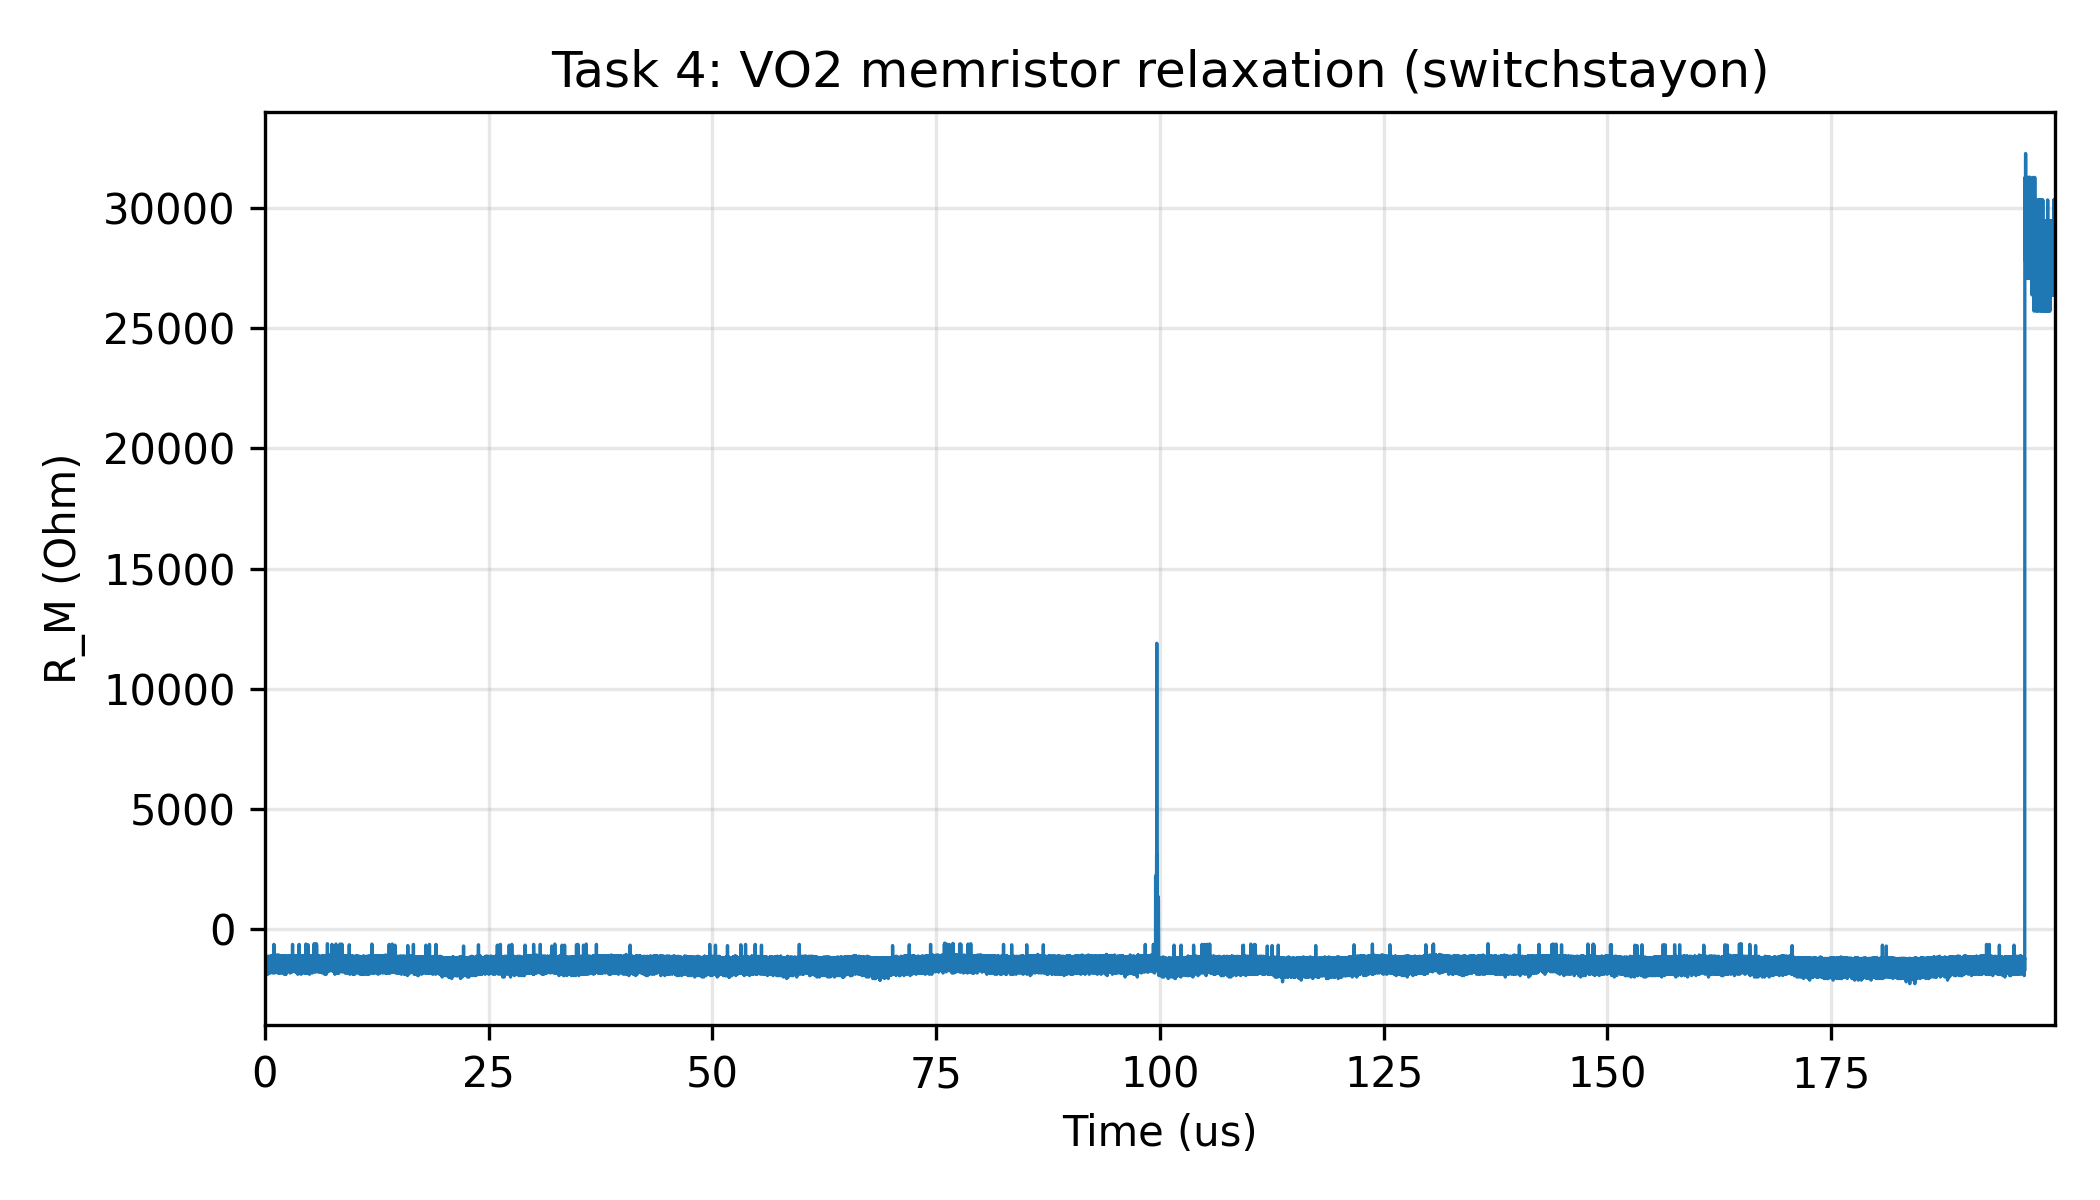
\includegraphics[width=0.65\linewidth]{task4_relaxation.png}
    \caption{Reconstructed memristor resistance during the reset experiment (Task 4) using \texttt{switchstayon.csv}. The relaxation to the high-resistance state completes after roughly \SI{197}{\micro\second}.}
    \label{fig:task4_relaxation}
\end{figure}

\subsection{Task 5: VO$_2$ Oscillator Outlook}

\begin{figure}[H]
    \centering
    \begin{subfigure}[b]{0.49\linewidth}
        \centering
        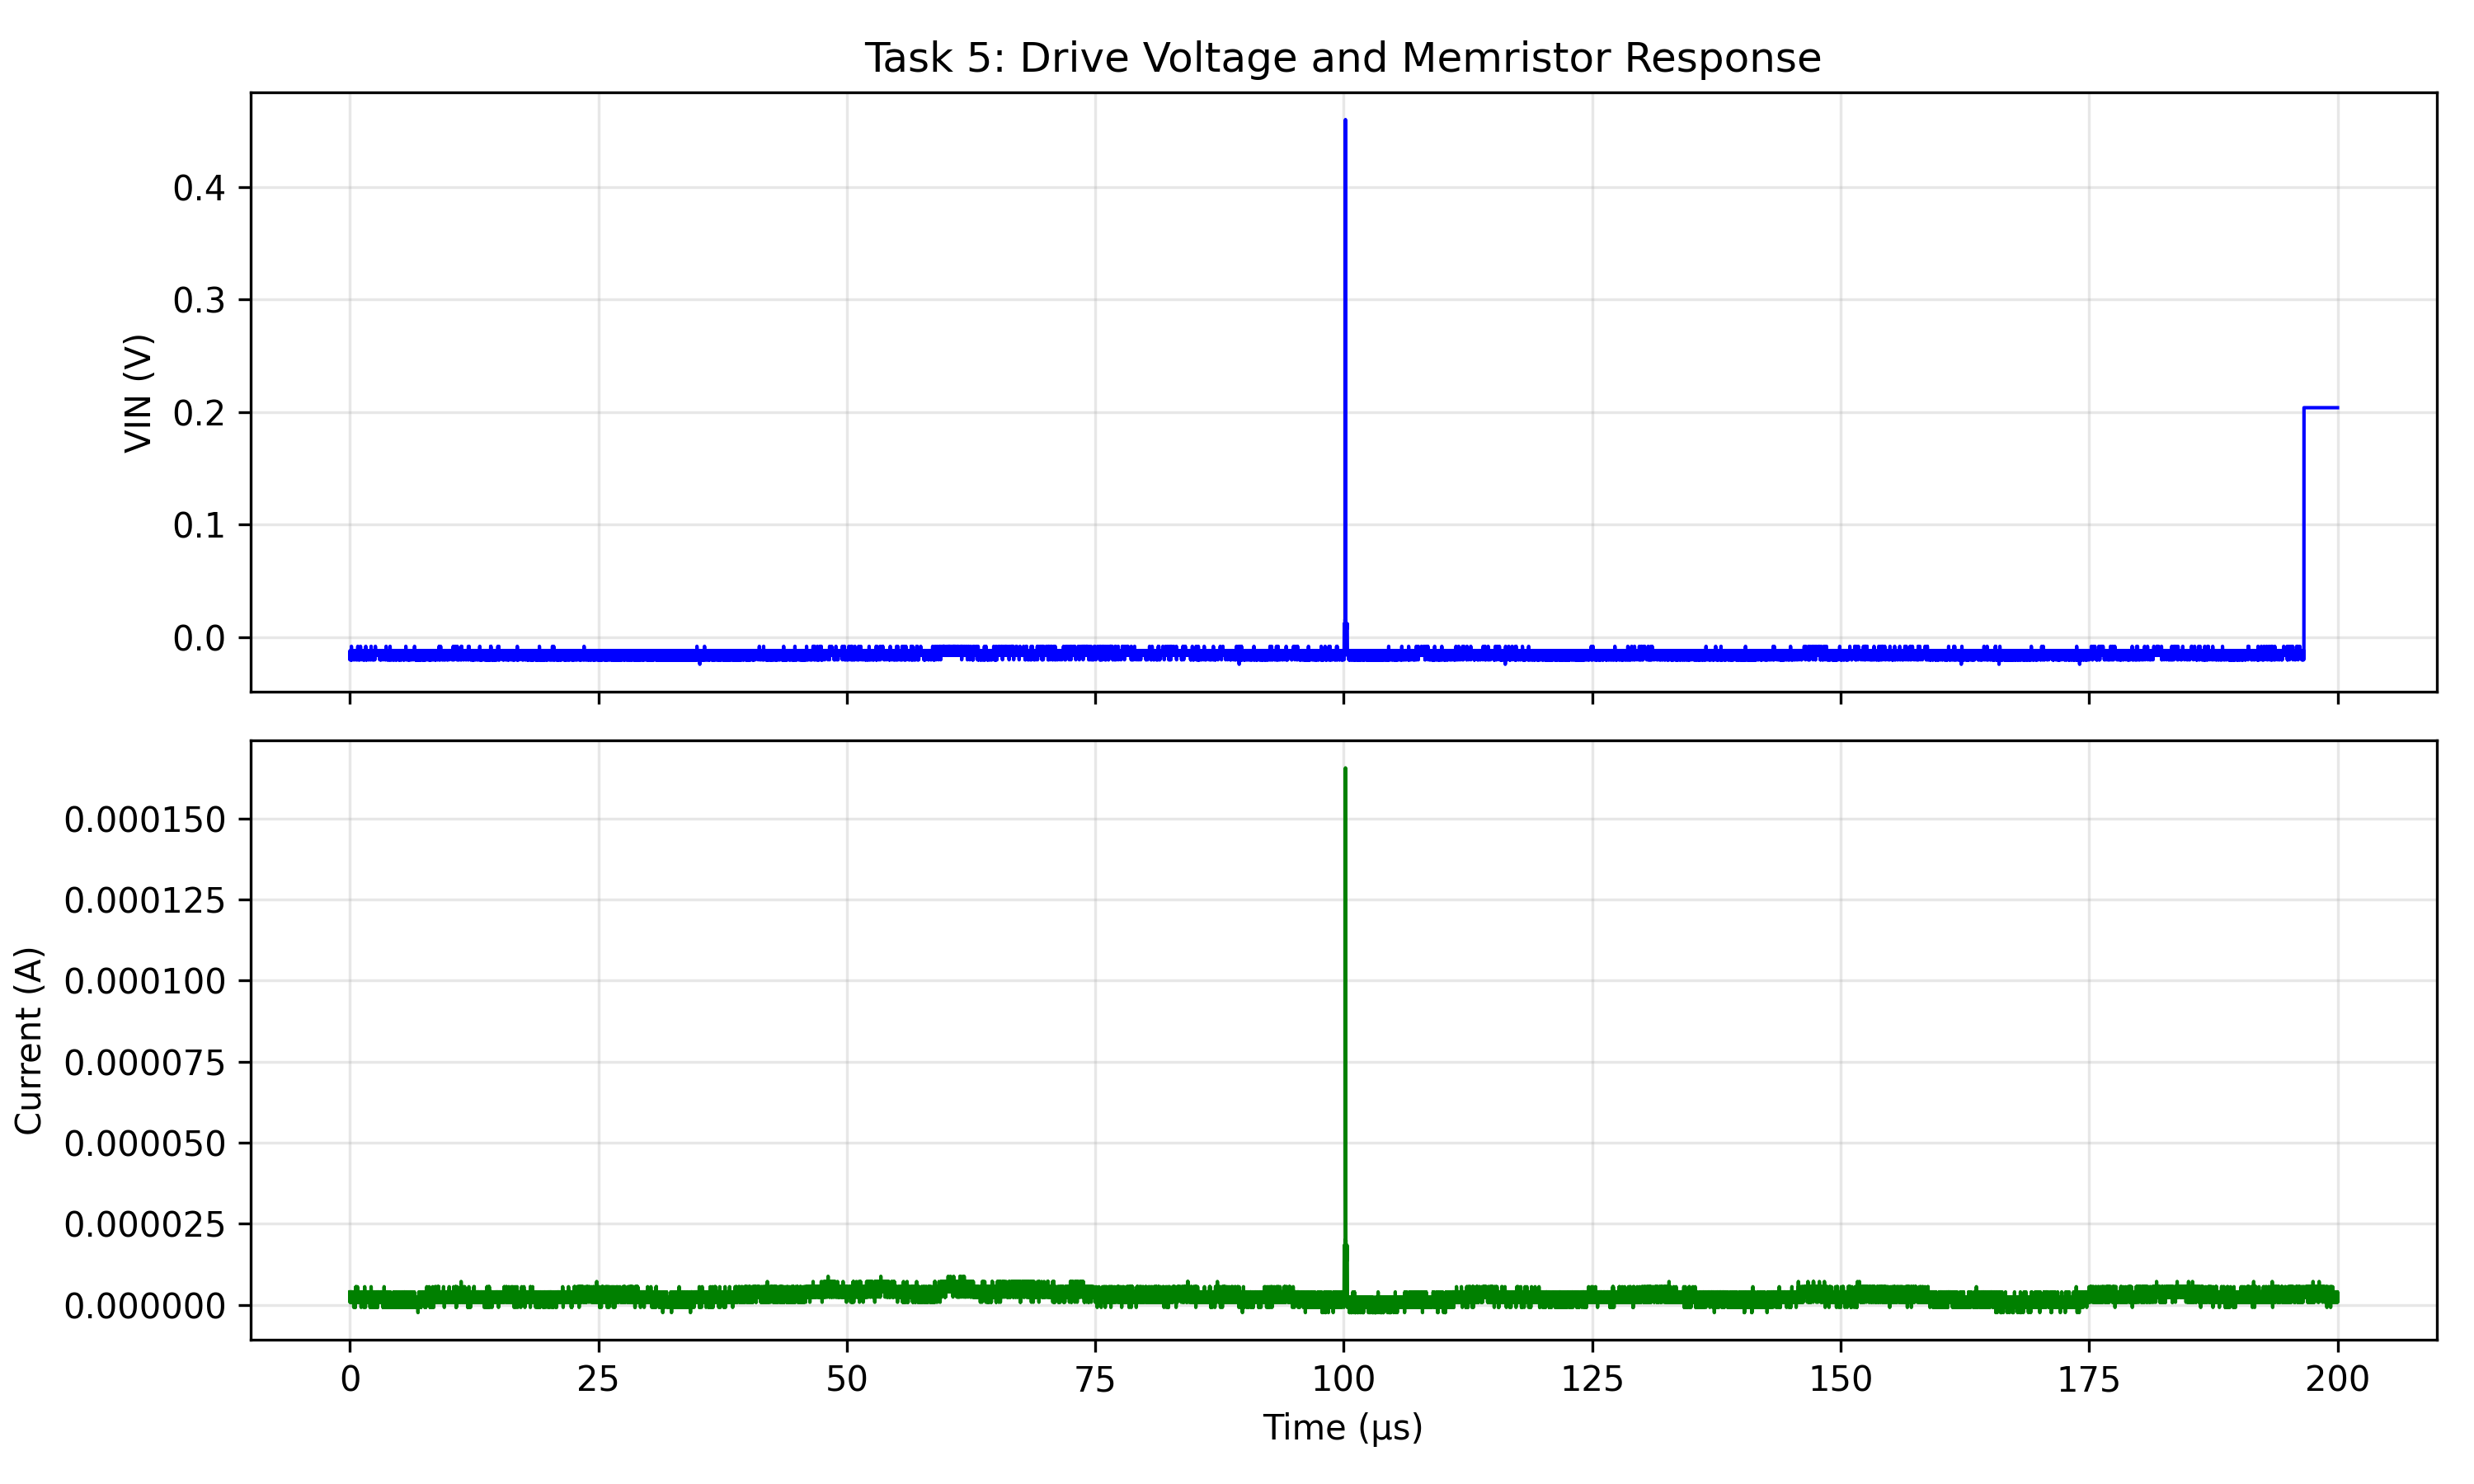
\includegraphics[width=\linewidth]{task5_full_trace.png}
        \caption{Full measurement window}
    \end{subfigure}
    \hfill
    \begin{subfigure}[b]{0.49\linewidth}
        \centering
        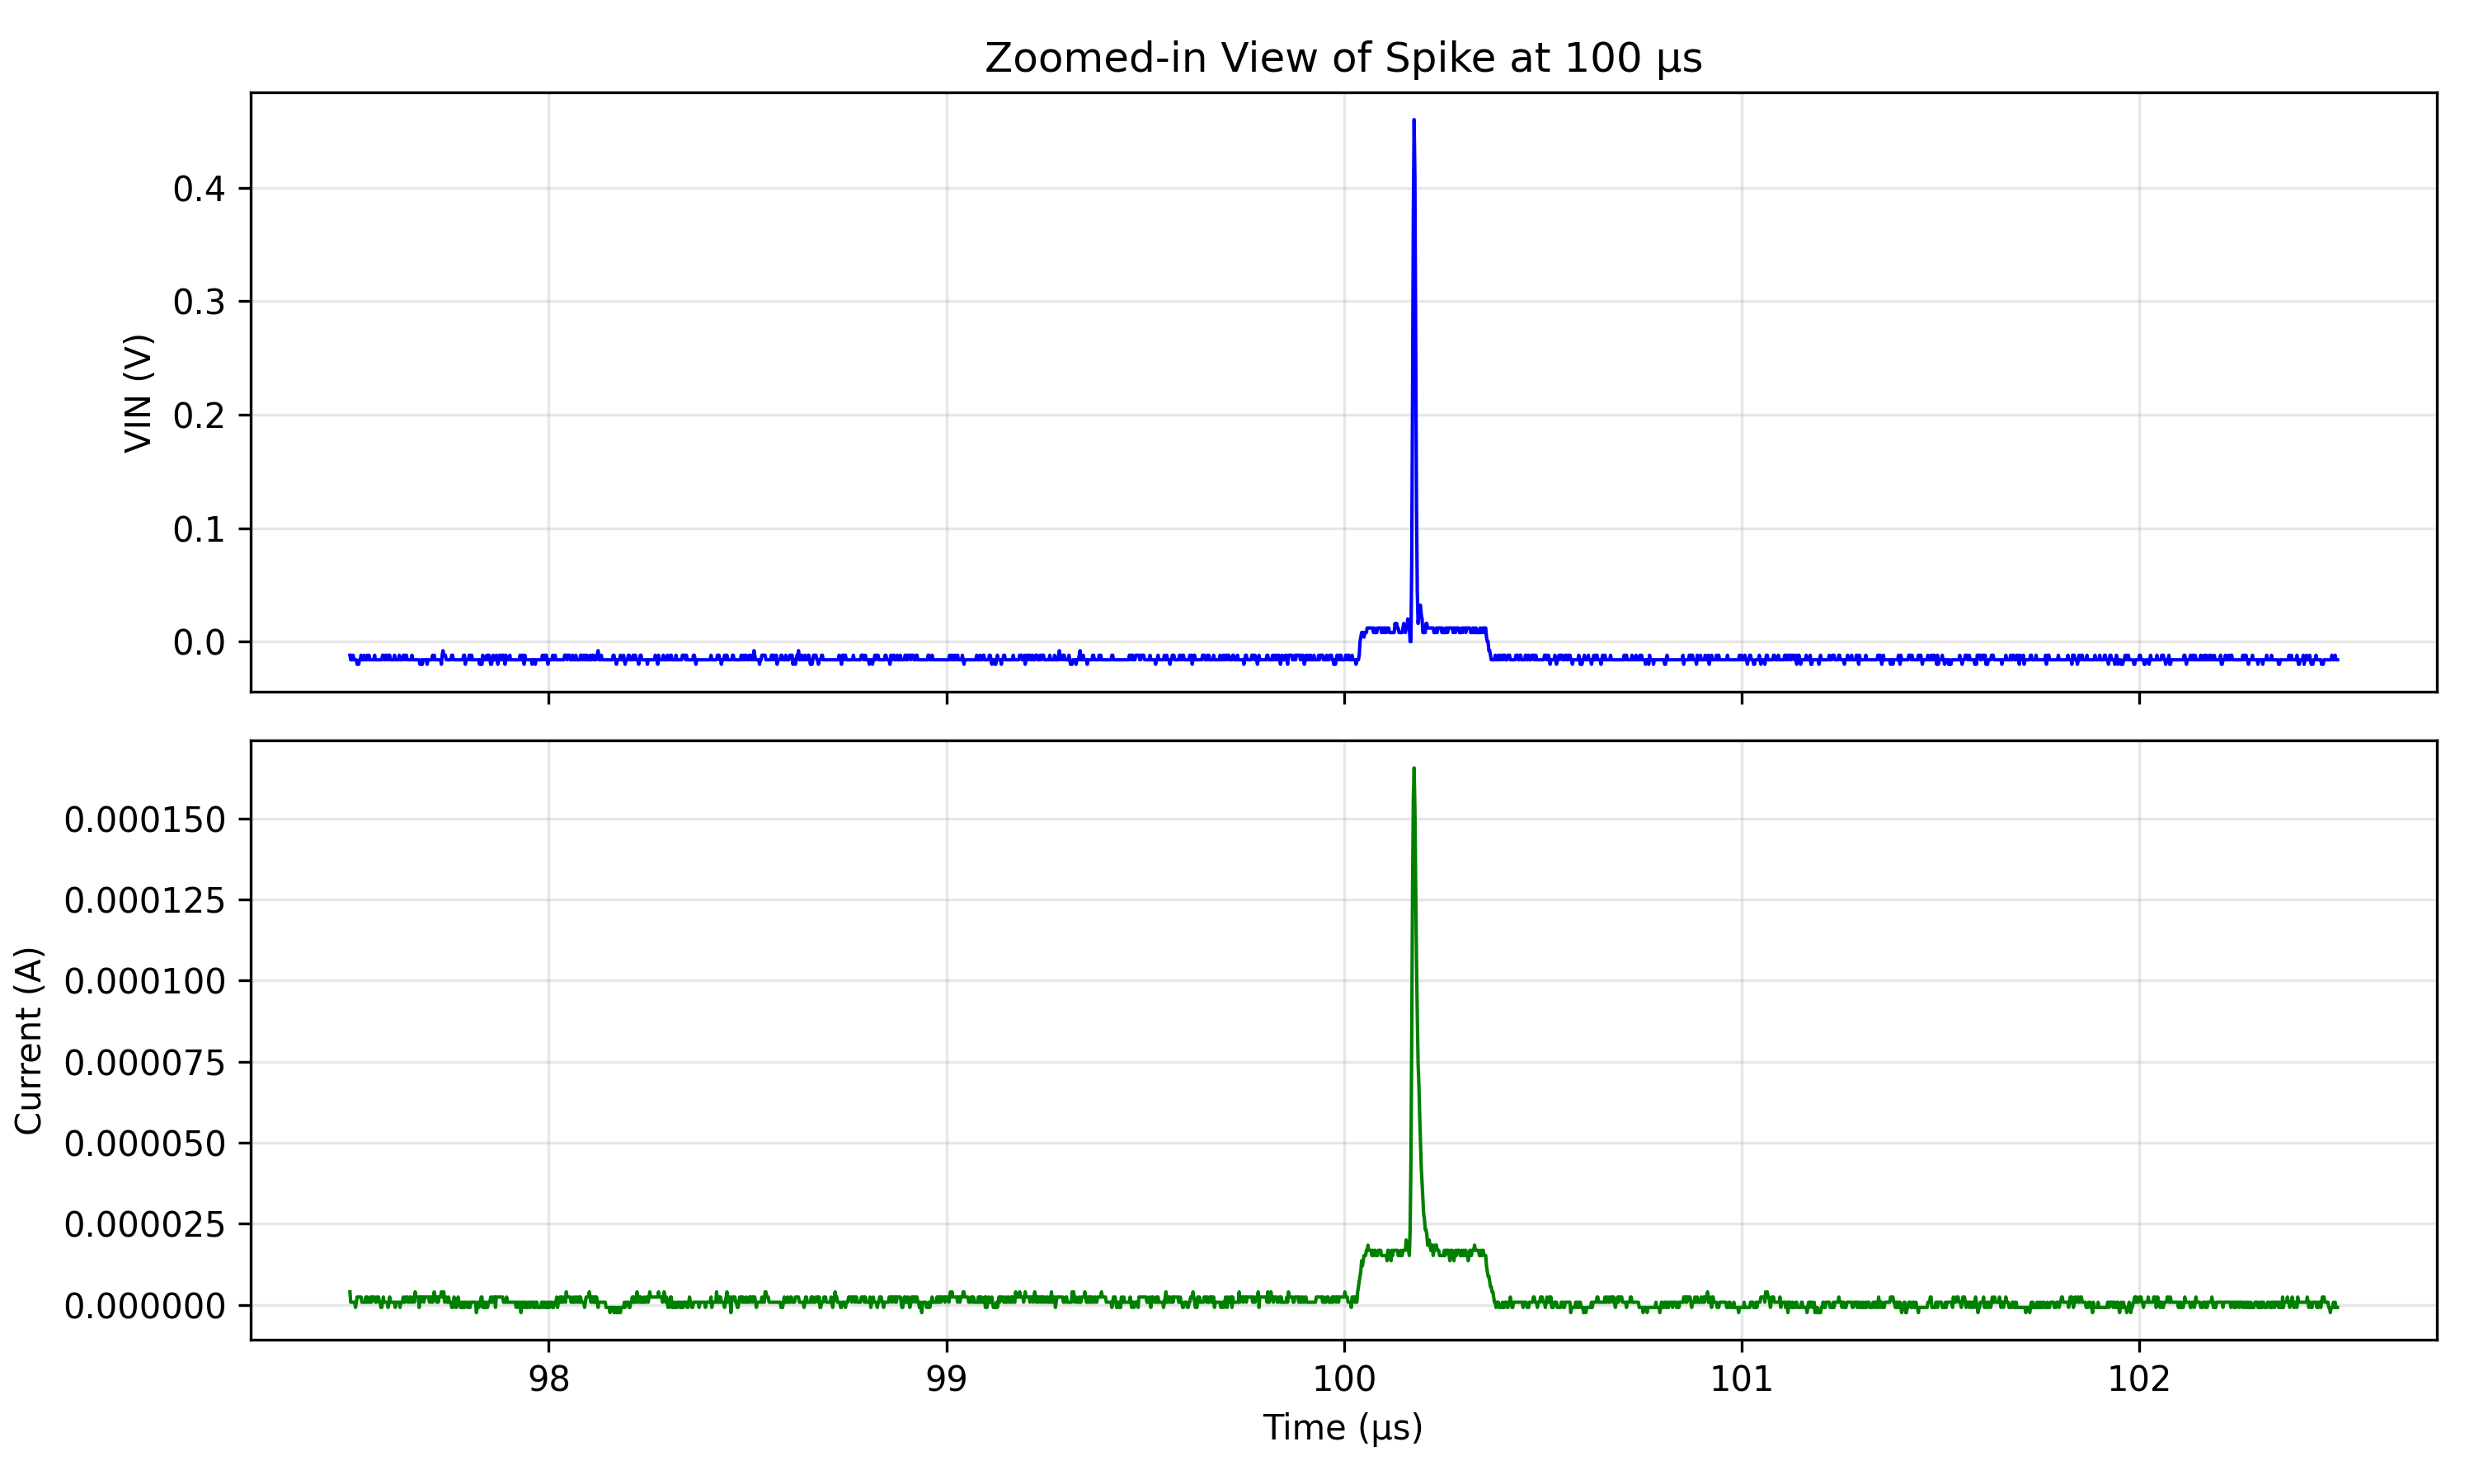
\includegraphics[width=\linewidth]{task5_zoom_spike.png}
        \caption{Zoomed-in view of the spike}
    \end{subfigure}
    \caption{Task 5 measurement from \texttt{short.csv}. The plots show that the circuit did not enter a self-sustaining oscillation. The current spike at \SI{\sim 100}{\micro\second} is a direct response to a drive voltage pulse, indicating the device acted as a switch rather than an oscillator.}
    \label{fig:task5_oscillator}
\end{figure}

The goal of this task was to create a self-sustaining oscillator. However, the data captured in \texttt{short.csv} shows that the circuit did not achieve stable oscillation (Figure~\ref{fig:task5_oscillator}). The current trace is mostly flat, with sharp spikes that directly correlate with pulses in the drive voltage. The zoomed-in view confirms that the current spike at \SI{\sim 100}{\micro\second} is a direct response to an input voltage pulse. This indicates that the conditions for oscillation were not met; the device behaved as a switch, but the circuit did not re-trigger itself. Frequency analysis (e.g., FFT) on this non-periodic signal would be misleading. This is a null result, suggesting that circuit parameters such as the drive voltage or series resistance would need further tuning to find an oscillation regime.

\subsection{Error Analysis}

Main sources of uncertainty: \textbf{Task 1:} Multimeter uncertainty \SI{\pm 1}{\percent} and SMD resistor tolerance \SI{\pm 1}{\percent} account for the \SI{0.8}{\percent} deviation. \textbf{Task 2:} DAQ voltage uncertainty \SI{\pm 0.1}{\percent}, series resistor tolerance \SI{\pm 1}{\percent}, and switching voltage variations due to thermal effects and device history. \textbf{Task 3:} PT1000 accuracy \SI{\pm 0.1}{\celsius}, thermal gradients from Peltier element, and contact resistance contributions. The R(T) hysteresis is physical, though its width may be affected by measurement rate. \textbf{Task 4:} Oscilloscope timing accuracy \SI{\pm 0.01}{\percent}, channel calibration errors \SI{\pm 1}{\percent} to \SI{\pm 3}{\percent}, channel phase mismatch causing negative resistance artifacts, \SI{50}{\ohm} termination tolerance \SI{\pm 1}{\percent}, and reset time extraction uncertainty \SI{\pm 5}{\micro\second} from noise. \textbf{Task 5:} Sampling rate requirements (Nyquist), peak detection sensitivity, FFT resolution $\Delta f = 1/T_{\text{window}}$, and load line stability affecting frequency.

\section{Conclusion}

The characterization of the VO$_2$ memristor successfully demonstrated the key properties required for neuromorphic applications. The I(V) measurements confirmed the volatile, hysteretic switching behavior, with clear set and reset voltages. The temperature-dependent resistance measurements revealed the insulator-metal phase transition around \SI{68}{\celsius}, consistent with known VO$_2$ properties.

The volatile nature of these devices, where they return to HRS at zero bias, makes them suitable for artificial neuron circuits. The combination of voltage-induced and temperature-induced switching provides multiple mechanisms for controlling the device state, enabling various neuromorphic computing architectures.

Future work could include detailed analysis of the relaxation dynamics (Task 4) to extract time constants, and investigation of oscillator circuits (Task 5) to demonstrate the device's potential for oscillating neural networks.

\appendix
\section{Data Processing Guide}
\label{sec:plot-guide}

The following procedures summarise the steps needed to regenerate every plot used (or still pending) in the report. The notebook \texttt{analyze\_memristor\_data.ipynb} contains reference code snippets for Tasks~2--5.

\subsection*{Task 1 -- Series Resistor Measurement}
\begin{enumerate}
    \item Load \texttt{task1.txt} (tab separated) and verify the columns for time, drive voltage, and measured node voltages.
    \item Compute the divider output using $V_{R_s}$ and confirm $R_s$ and $R_{\text{smd}}$ via $R=V/I$.
    \item Plot the raw time series of the measured voltages to produce Figure~\ref{fig:task1_timeseries}.
    \item Fit the linear transfer characteristic (output vs input) to obtain the gradient corresponding to the resistor ratio, and export Figure~\ref{fig:task1_fit}.
\end{enumerate}

\subsection*{Task 2 -- I(V) Sweep}
\begin{enumerate}
    \item Load \texttt{task2\_second} (tab separated). Use $R_s=\SI{2.17}{\kilo\ohm}$.
    \item Derive the current $I=V_{R_s}/R_s$ and the memristor bias $V_{\text{bias}}=V_{\text{drive}}-I R_s$.
    \item Generate the time-domain traces of $V_{\text{drive}}$, $V_{R_s}$, and $I$ (Figure~\ref{fig:task2_three_plots}).
    \item Plot $I$ versus $V_{\text{bias}}$ to obtain the hysteretic I(V) curve (Figure~\ref{fig:task2_memristor_iv}); optionally fit linear segments to estimate differential resistance.
\end{enumerate}

\subsection*{Task 3 -- Temperature-Dependent Resistance}
\begin{enumerate}
    \item Load \texttt{task3.csv} and extract the columns ``Temperature (C)'' and ``Sample Resistance (Ohm)''.
    \item Separate the heating and cooling branches by monitoring the monotonicity of the temperature column (or by splitting at the maximum temperature).
    \item Plot $R$ vs $T$ on a semi-logarithmic scale, using different colours/markers for heating and cooling to show hysteresis.
    \item Mark the transition temperature (e.g., where $\mathrm{d}R/\mathrm{d}T$ peaks) and export the figure (to be saved as \texttt{task3\_rt.png}).
\end{enumerate}

\subsection*{Task 4 -- Relaxation (Reset) Dynamics}
\begin{enumerate}
    \item Load \texttt{switchstayon.csv}. Convert CH2 and CH1 from millivolts to volts and create the time axis using the \SI{2}{\nano\second} sampling interval (information in the file header).
    \item Mask samples where $|V_{\text{trans}}|<\SI{1}{\milli\volt}$ to avoid division noise, then compute $R_M(t)=2Z_0\left(\nicefrac{V_{\text{in}}}{V_{\text{trans}}}-1\right)$ with $Z_0=\SI{50}{\ohm}$.
    \item Plot $R_M$ versus time in microseconds, annotate the low- and high-resistance plateaus, and extract the $90\,\%$ reset time (\SI{\sim 197}{\micro\second}). Save as \texttt{task4\_relaxation.png}.
\end{enumerate}

\subsection*{Task 5 -- VO$_2$ Oscillator}
\begin{enumerate}
    \item Export the oscilloscope acquisition with columns for time, shunt voltage $V_{\text{trans}}$, and drive voltage $V_{\text{in}}$ (CSV format).
    \item Update Cell~6 in \texttt{analyze\_memristor\_data.ipynb} with the file path and column names.
    \item Compute the current $I(t)=V_{\text{trans}}/Z_0$, plot $V_{\text{in}}$ and $I$ versus time, and determine the oscillation frequency using peak detection or FFT.
    \item Summarise the frequency versus drive amplitude (or capacitance) if multiple sweeps are available, and export the waveform/frequency plots for inclusion in the report.
\end{enumerate}

\section{Supplementary Photos}

\begin{figure}[H]
    \centering
    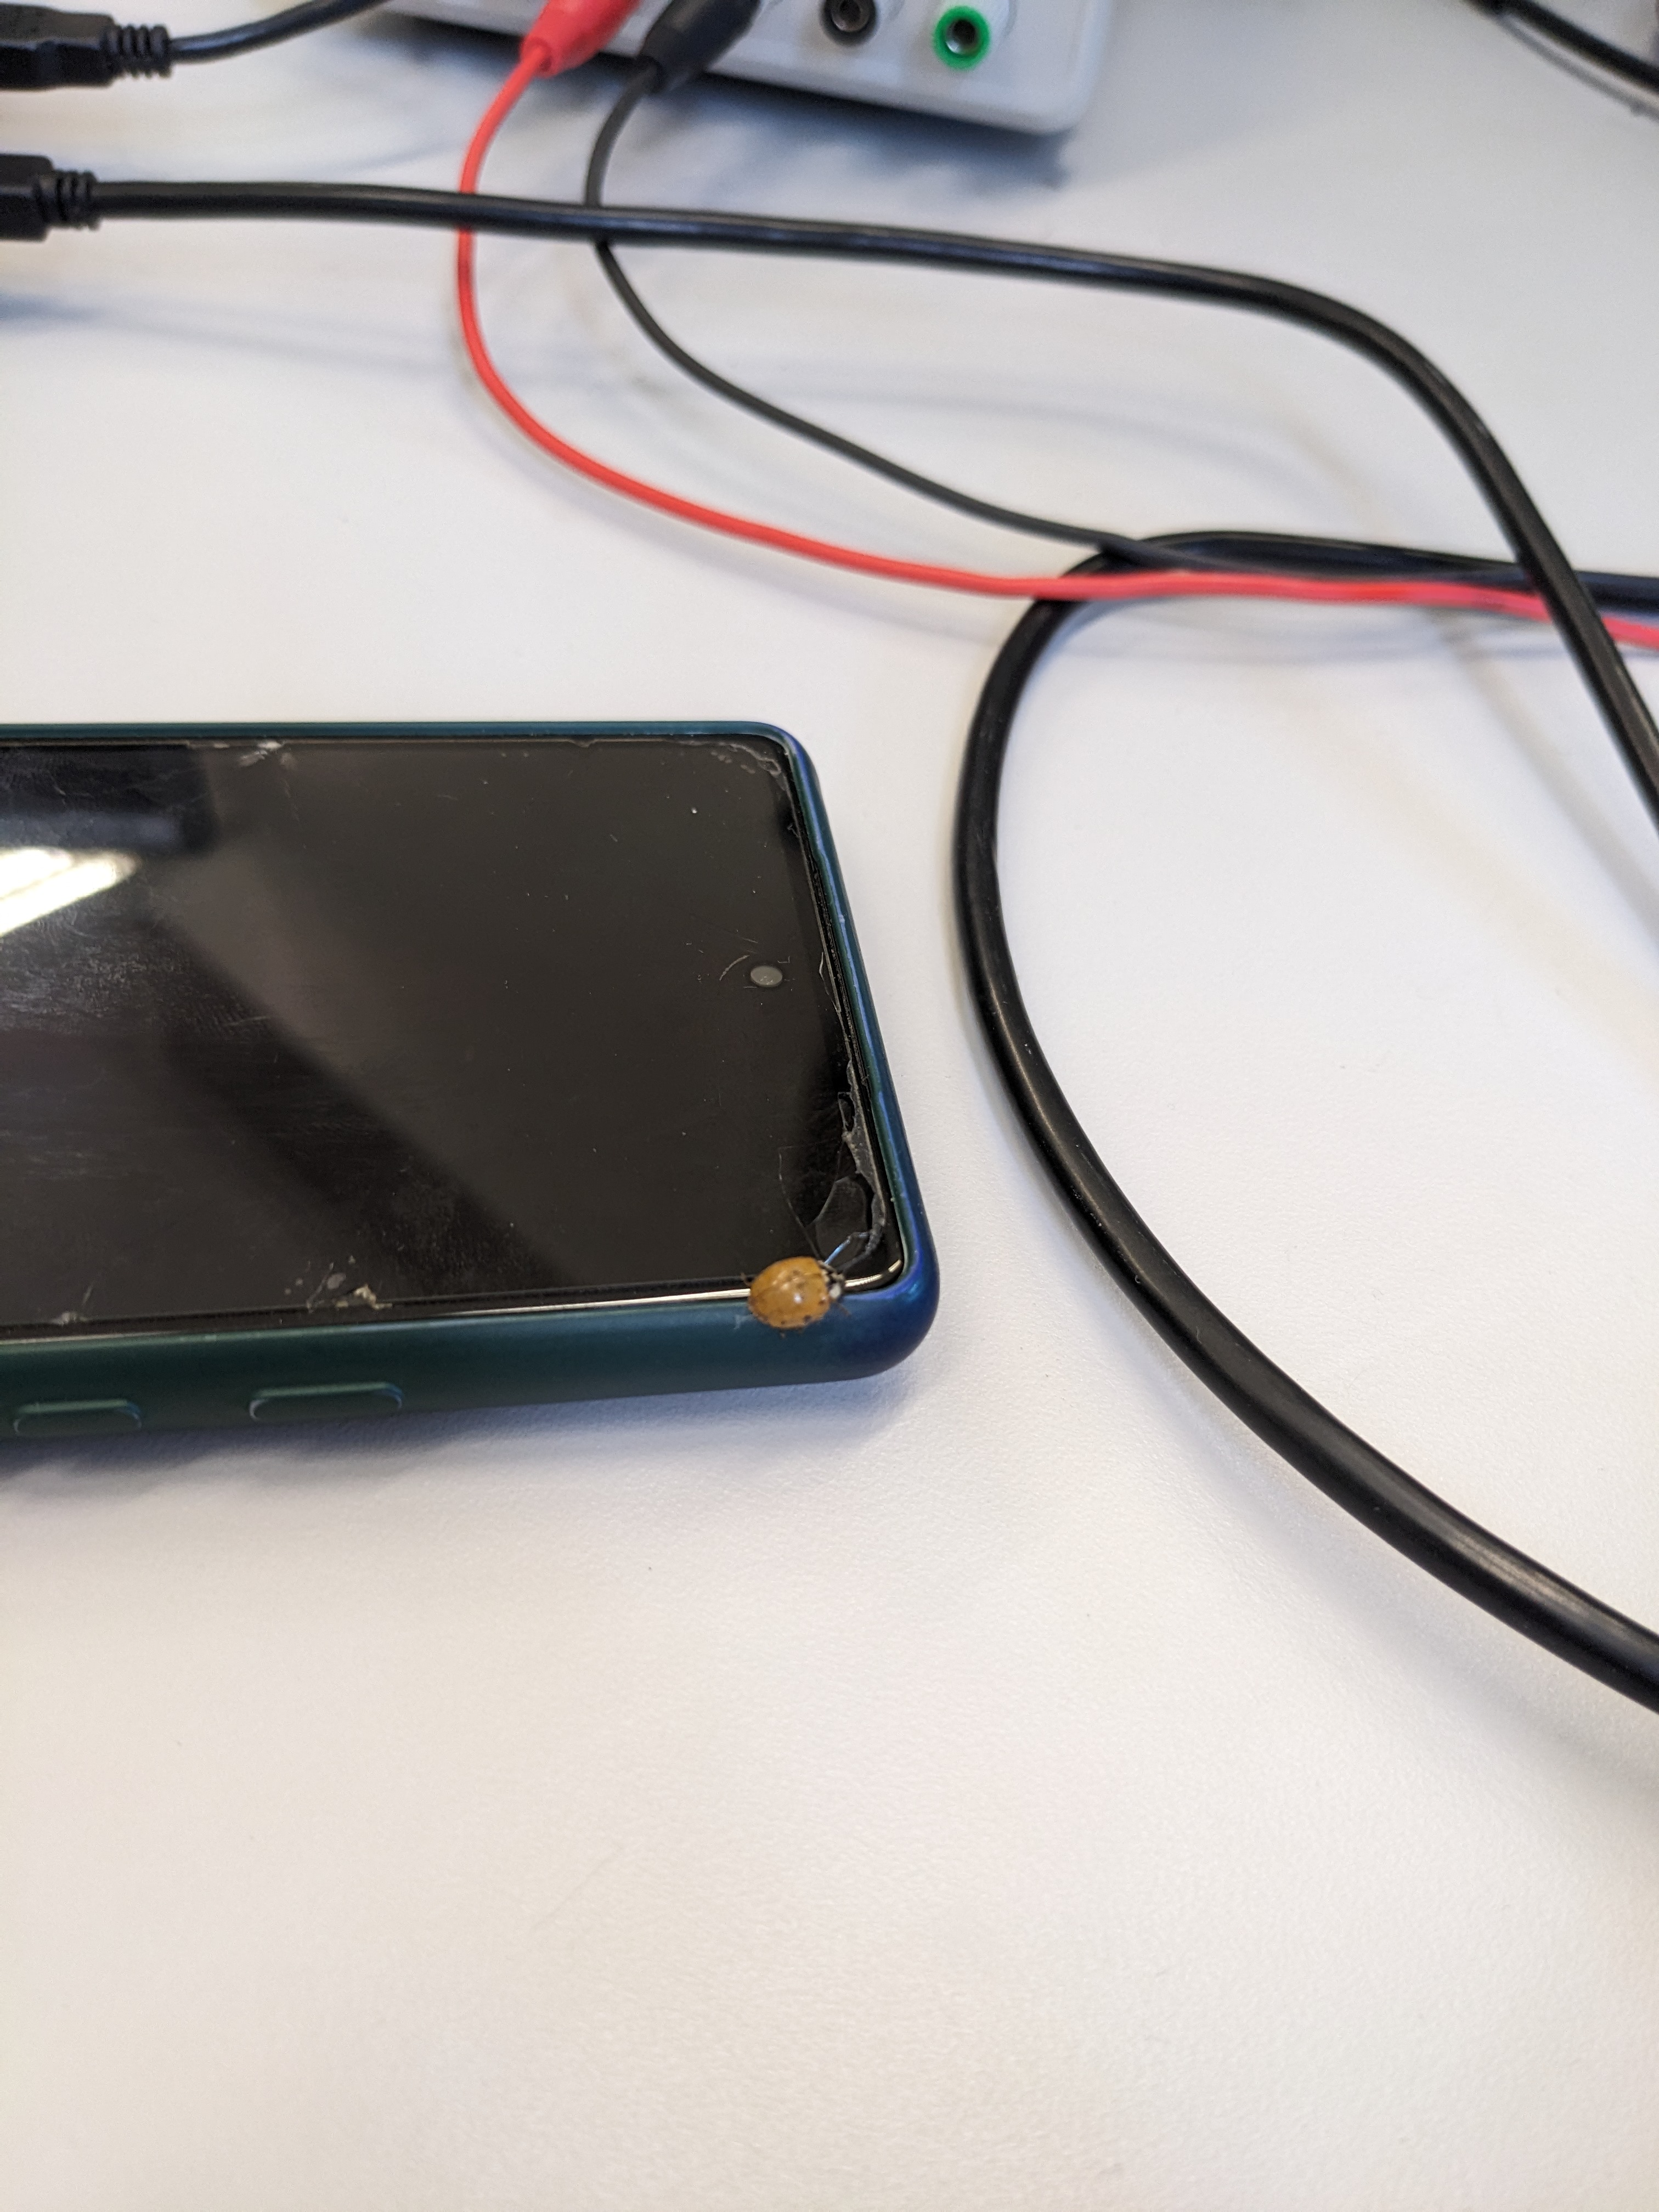
\includegraphics[width=0.6\linewidth]{photos/PXL_20251030_132836538.MP.jpg}
    \caption{Ladybug observed on Grego's phone during preparation.}
    \label{fig:ladybug}
\end{figure}

\end{document}
